% 第三章 Hopfion 稳定性研究
\chapter{Hopfion 稳定性研究}

本章聚焦两类磁性介质中 Hopfion 的存活条件：含体积型 DMI 的铁磁体（以 FeGe 为代表材料）与竞争交换铁磁体。借助微磁学仿真，本文逐一勘定两套体系中 Hopfion 得以维持的必要前提及可行参数窗口。


\section{DMI 铁磁体系中的 Hopfion 稳定性}

\par\noindent\textbf{FeGe 材料参数与模型设置}\par\nobreak

研究对象选为手性磁体 FeGe，其材料参数见\cref{tab:fege-params}。由 $\lambda = 4\pi A_{\text{ex}} / |D_{\text{bulk}}| \approx \SI{70}{nm}$ 给出的螺旋周期构成体系固有的空间标度，模型几何尺寸的选取也以此为基准。

\begin{table}[htbp]
  \centering
  \caption{FeGe 材料参数}
  \label{tab:fege-params}
  \begin{tabular}{lll}
    \toprule
    参数 & 符号 & 数值 \\
    \midrule
    饱和磁化强度 & $M_s$ & $\SI{384e3}{A/m}$ \\
    交换刚度 & $A_{\text{ex}}$ & $\SI{8.78e-12}{J/m}$ \\
    体积型 DMI 常数 & $D_{\text{bulk}}$ & $\SI{1.58e-3}{J/m^2}$ \\
    螺旋周期 & $\lambda$ & $\SI{70}{nm}$ \\
    \bottomrule
  \end{tabular}
\end{table}

几何上取圆柱体，直径 $d = \SI{210}{nm} = 3\lambda$，厚度 $h = \SI{70}{nm} = \lambda$。离散网格取 $\SI{1}{nm} \times \SI{1}{nm} \times \SI{1}{nm}$，足以分辨该材料的交换长度。

\par\noindent\textbf{初始态构造：Sutcliffe 解析解}\par\nobreak

Hopfion 的初始磁化构型依据 Sutcliffe 给出的解析形式\cite{sutcliffe2018hopfions}生成。该解建立在有理映射近似之上，可直接给出拓扑荷 $Q_H = 1$ 的磁化分布。具体流程是用 Python 脚本计算该解析构型，导出为 OVF 文件，再交由 Mumax3 读入。

进入 Hopfion 的核心区域后，$m_z$ 的走向为：中心管内 $-1$（反向磁化通道），向外渐变至 $+1$（均匀背景），中间环形过渡区呈现旋转结构。

\par\noindent\textbf{稳定性的三个必要条件}\par\nobreak

通过对比实验，本文梳理出 FeGe 体系里 Hopfion 能够稳定存在的三条必要条件：

\textbf{条件一：解析初始态。} 随机初始化或简单的环形（torus）初始化均无法让系统落入 Hopfion 亚稳态。只有当起点取自 Sutcliffe 解析构型，磁化分布才位于 Hopfion 能量盆地的吸引域以内。

\textbf{条件二：边界层冻结。} 圆柱模型顶面与底面的边界层磁化被固定在 $\mathbf{m} = \hat{z}$，由 Mumax3 的 \texttt{frozenspins} 特性实现。一旦放开这层约束，DMI 往往会在边界处诱发螺旋态，使 Hopfion 所依赖的均匀背景无法维持。

\textbf{条件三：退磁场效应。} 退磁场计算（\texttt{EnableDemag = true}）必须开启。该项贡献一份额外的形状各向异性，有助于稳住 $m_z = +1$ 背景，从而支撑起 Hopfion 的空间构型。

各条件组合下的仿真结果汇总于\cref{tab:fege-conditions}。

\begin{table}[htbp]
  \centering
  \caption{FeGe 体系中 Hopfion 稳定条件的对比实验}
  \label{tab:fege-conditions}
  \begin{tabular}{cccc}
    \toprule
    解析初始态 & 边界冻结 & 退磁场 & 结果 \\
    \midrule
    \checkmark & \checkmark & \checkmark & 稳定（2 ns） \\
    \checkmark & \checkmark & $\times$   & 螺旋态 \\
    \checkmark & $\times$   & \checkmark & 螺旋态 \\
    $\times$   & \checkmark & \checkmark & 不收敛 \\
    \bottomrule
  \end{tabular}
\end{table}

\par\noindent\textbf{弛豫与演化结果}\par\nobreak

在三条必要条件同时满足的前提下，本文先以 $\alpha = 0.5$ 的高阻尼做 Relax 弛豫，把初始态推入局部能量极小值；再切换到 $\alpha = 0.02$ 做 \SI{2}{ns} 时间演化。仿真显示 Hopfion 持续稳定，$\langle m_z \rangle = 0.376$，核心半径约 \SI{50}{nm}。

\cref{fig:fege-stable}给出弛豫完成后 Hopfion 的稳态形貌。左图为 $z = 0$ 中平面的 $m_z$ 分布，可清晰辨认出中心反向磁化区（$m_z = -1$，深蓝色）与环形过渡层；中图取 $y = 0$ 截面，呈现 Hopfion 沿 $z$ 轴延伸的管状核心；右图展示面内磁化分量，呈现出 Bloch 型的旋转特征。

\begin{figure}[htbp]
  \centering
  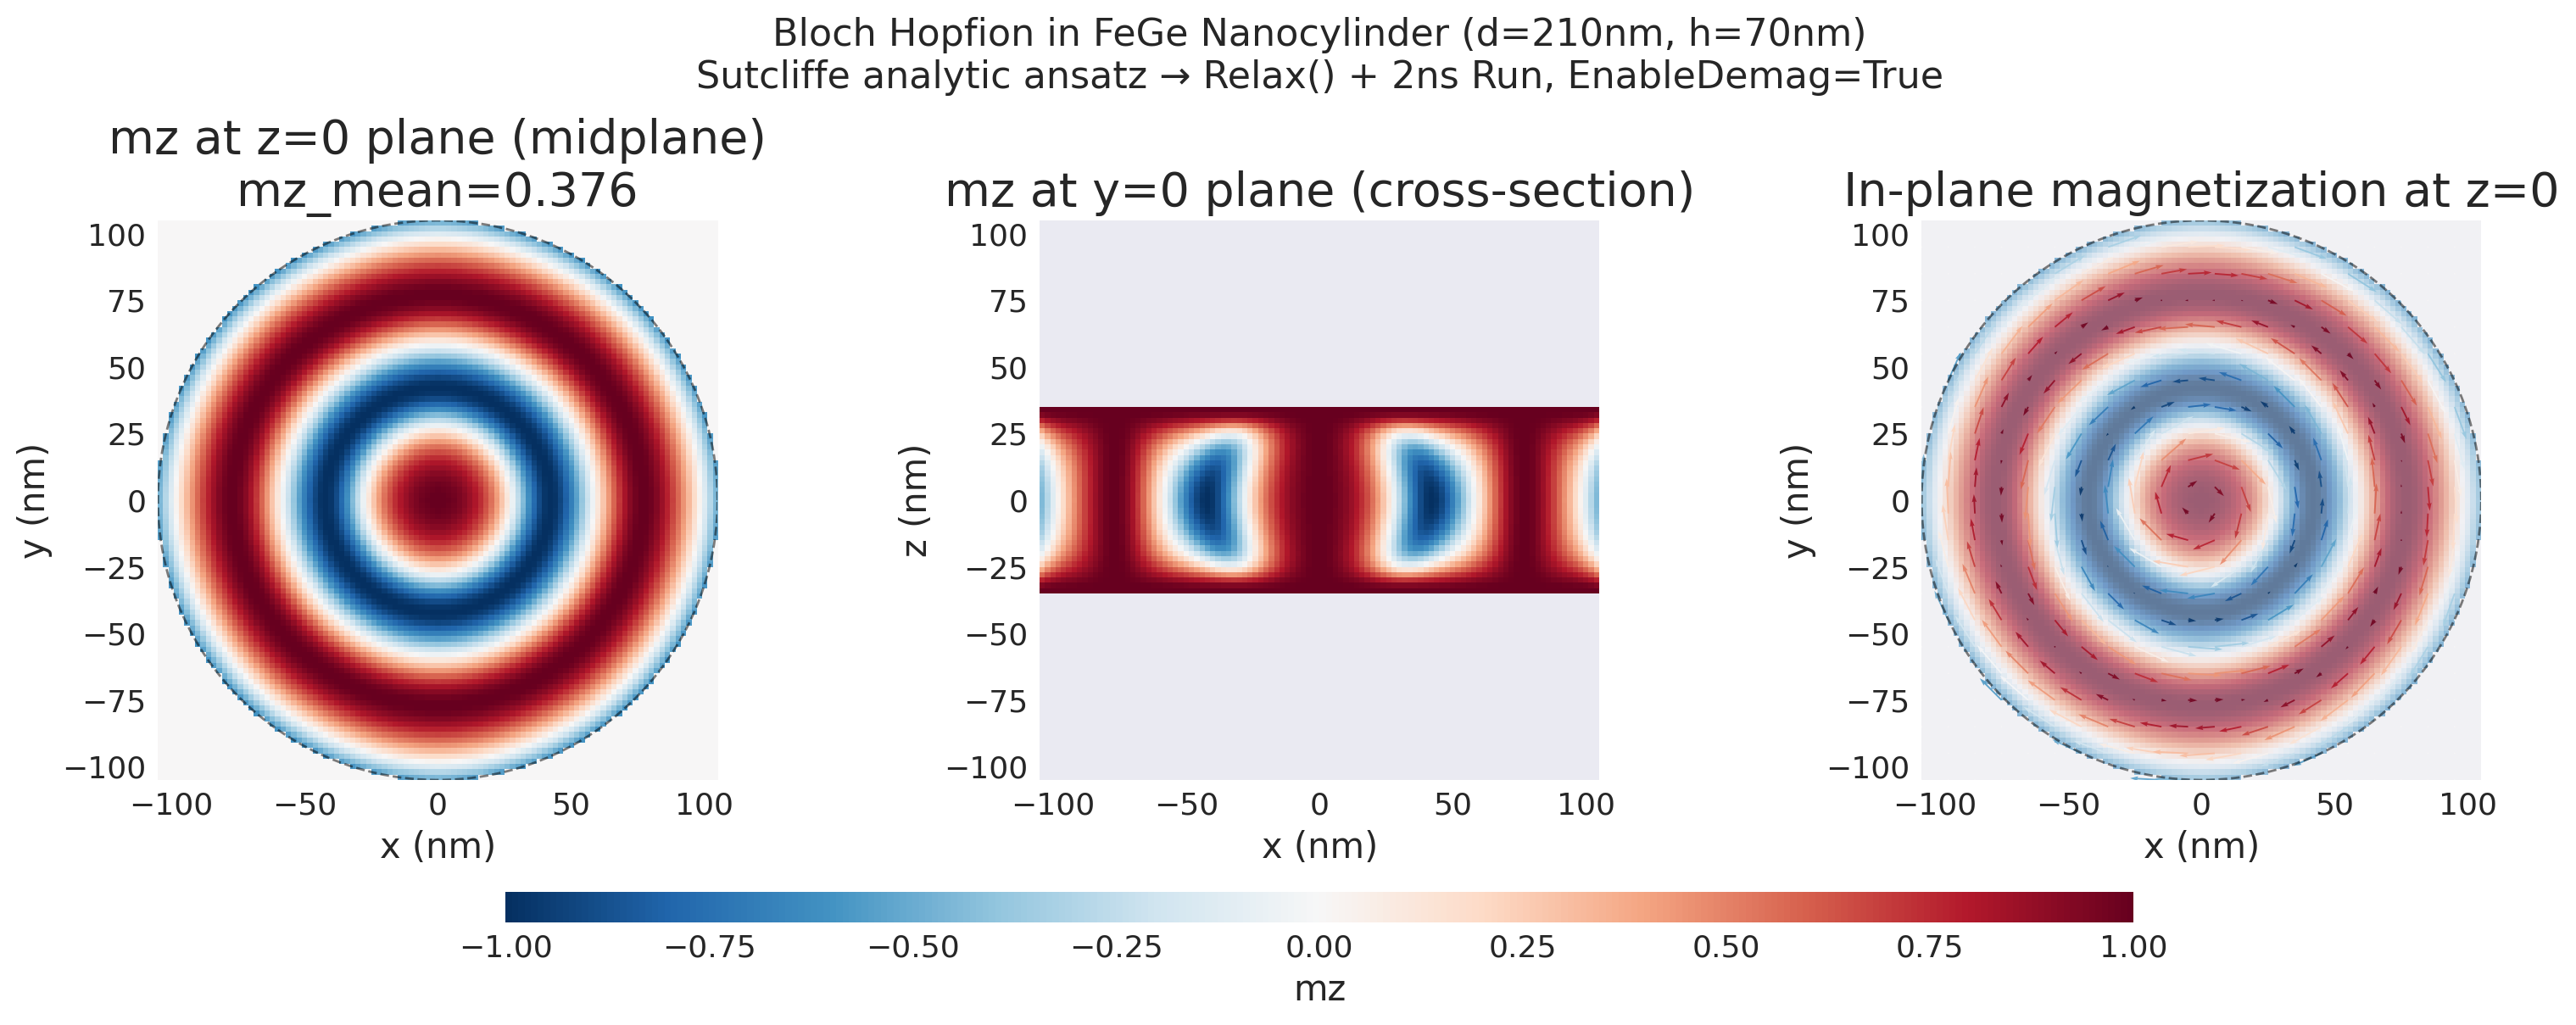
\includegraphics[width=0.95\textwidth]{figures/fig3-1_fege_hopfion_stable.png}
  \caption{FeGe 体系中 Bloch 型 Hopfion 经弛豫和 \SI{2}{ns} 时间演化后的稳态结构。左：$z = 0$ 中平面 $m_z$ 分布（$\langle m_z \rangle = 0.376$）；中：$y = 0$ 截面；右：面内磁化分量}
  \label{fig:fege-stable}
\end{figure}


\section{竞争交换铁磁体系中的 Hopfion 稳定性}

\par\noindent\textbf{模型设置}\par\nobreak

竞争交换铁磁体系的切入点来自 Sallermann 等的理论研究\cite{sallermann2023stability}。沿着该线索，Lobanov 与 Uzdin 剖析了此类体系中 Hopfion 的寿命、坍塌通道和逃逸机制\cite{lobanov2023lifetime}。模型所用参数列于\cref{tab:frustrated-params}。

\begin{table}[htbp]
  \centering
  \caption{竞争交换铁磁体系参数}
  \label{tab:frustrated-params}
  \begin{tabular}{lll}
    \toprule
    参数 & 符号 & 数值 \\
    \midrule
    饱和磁化强度 & $M_s$ & $\SI{1.5e5}{A/m}$ \\
    最近邻交换刚度 & $A_{\text{ex}}$ ($J_1$) & $\SI{5e-12}{J/m}$ \\
    次近邻交换 & $J_2$ & $-0.164 \, J_1$ \\
    第四近邻交换 & $J_4$ & $-0.082 \, J_1$ \\
    模型尺寸 & — & $\SI{50}{nm} \times \SI{50}{nm} \times \SI{50}{nm}$ \\
    网格 & — & $100 \times 100 \times 100$ \\
    格点间距 & — & $\SI{0.5}{nm}$ \\
    边界条件 & — & 三维周期性边界 \\
    \bottomrule
  \end{tabular}
\end{table}

相较 DMI 体系，此处关掉了 DMI、磁晶各向异性与退磁场三项，Hopfion 的存活只靠竞争交换一项支撑。为模拟无限大体块材料，本文启用三维周期性边界条件（PBC）。

\par\noindent\textbf{漂移稳定性分析}\par\nobreak

均匀背景中的 Hopfion 是否会自发漂移，直接关系到其作为器件载体的可行性。为此本文在严格控制变量的条件下（统一 $\alpha = 0.2$、$K_{u1} = 0$、相同初始尺寸 $R = \SI{3}{nm}$, $r = \SI{2}{nm}$、运行时长 \SI{2}{ns}）组织了四组对照实验，覆盖不同背景磁化方向（$m_z$、$m_x$、$m_y$）与 Hopfion 轴向（$z$、$x$、$y$ 三轴）的搭配。

漂移实验的数据汇总见\cref{tab:drift-results}。从仿真结果看，\textbf{四组配置表现出高度一致的行为}：Hopfion 质心在最初 $\sim\SI{1}{ns}$ 内沿环面轴向完成 $\approx \SI{4.75}{nm}$ 的一次性位移，之后即告钉扎；任何垂直于该轴向的分量始终为零。由此判断，背景磁化的取向对 Hopfion 漂移模式并无影响。

\begin{table}[htbp]
  \centering
  \caption{控制变量漂移实验结果汇总（统一参数：$\alpha = 0.2$, $K_{u1} = 0$, $R_0 = \SI{3}{nm}$, $r_0 = \SI{2}{nm}$）}
  \label{tab:drift-results}
  \begin{tabular}{ccccc}
    \toprule
    配置 & 背景方向 & Hopfion 轴向 & 轴向位移 & 横向位移 \\
    \midrule
    bg=$m_z$, axis=$z$ & $m_z = +1$ & $z$ & $+\SI{4.75}{nm}$ ($z$) & $\SI{0}{nm}$ \\
    bg=$m_z$, axis=$x$ & $m_z = +1$ & $x$ & $+\SI{4.75}{nm}$ ($x$) & $\SI{0}{nm}$ \\
    bg=$m_y$, axis=$y$ & $m_y = +1$ & $y$ & $+\SI{4.75}{nm}$ ($y$) & $\SI{0}{nm}$ \\
    bg=$m_x$, axis=$x$ & $m_x = +1$ & $x$ & $+\SI{4.75}{nm}$ ($x$) & $\SI{0}{nm}$ \\
    \bottomrule
  \end{tabular}
\end{table}

需要指出，这个 \SI{4.75}{nm} 轴向位移来源于初始态在离散格点上的弛豫过程。连续的解析 ansatz 落到格点体系后，质心需要滑移到最近的格点势极小处；这一迁移在约 \SI{1}{ns} 内结束，随后格点势将 Hopfion 牢牢锁住。位移之所以严格沿环面轴向，是因为该方向的势垒较浅，而环面平面内的钉扎势深度明显更大。

四组实验的总漂移距离对比参见\cref{fig:drift-comparison}。曲线在误差范围内几乎完全重合，再次印证了前述结论。本文选取 $m_x = +1$ 背景作 \SI{10}{ns} 长时验证（\cref{fig:drift-10ns}）：Hopfion 在完成初始弛豫后的 \SI{9}{ns} 内质心完全静止，$y$、$z$ 两方向全程零漂移，长时稳定性得到进一步确认。

\begin{figure}[htbp]
  \centering
  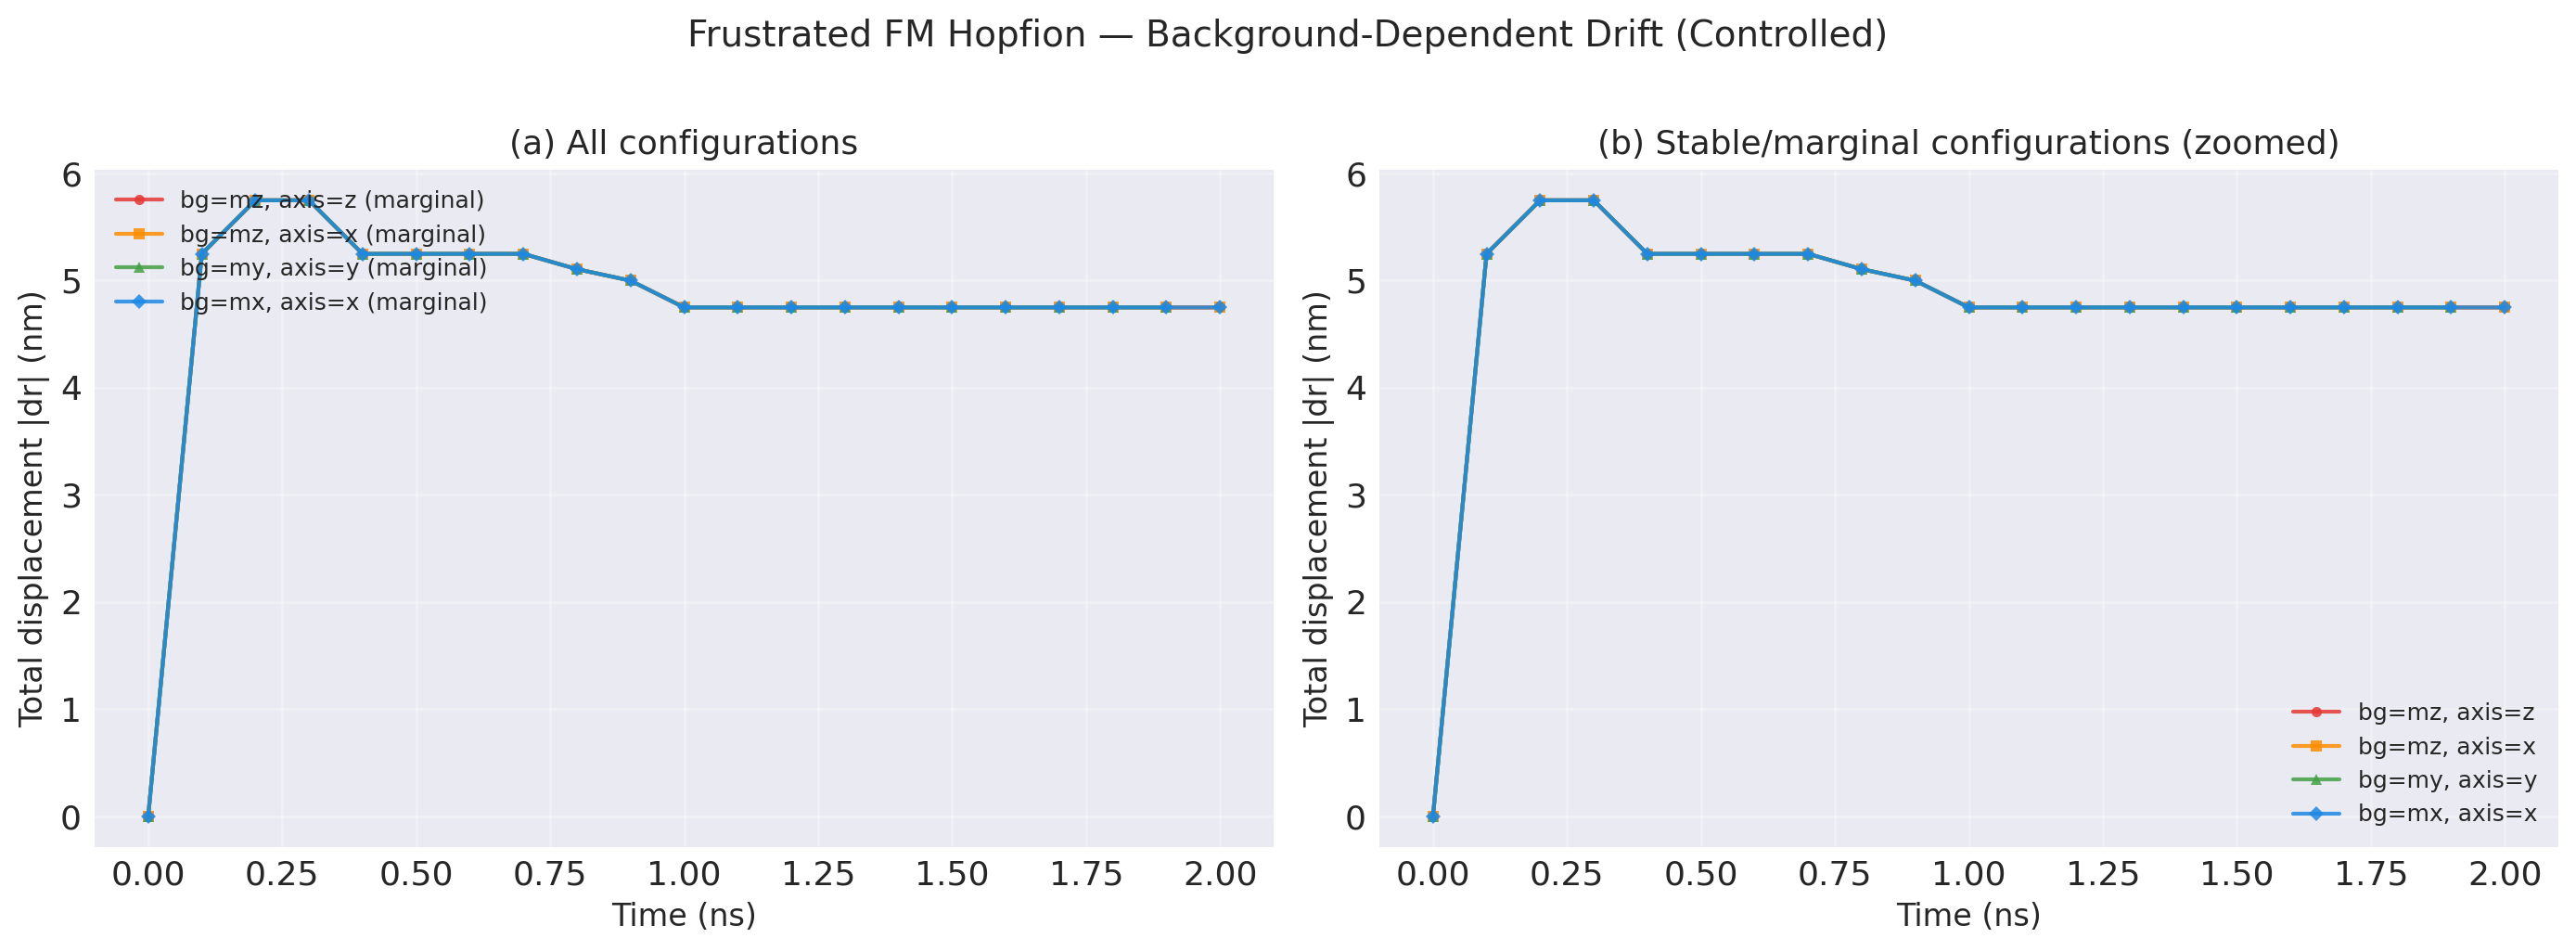
\includegraphics[width=0.95\textwidth]{figures/fig3-4_drift_comparison.png}
  \caption{四组配置的总漂移距离 $|\Delta r|$ 随时间的演化。所有曲线完全重合：前 $\sim\SI{1}{ns}$ 内质心因格点弛豫沿轴向位移 $\approx\SI{4.75}{nm}$，此后完全钉扎。背景磁化方向（$m_z$、$m_x$、$m_y$）对漂移行为无影响}
  \label{fig:drift-comparison}
\end{figure}

\begin{figure}[htbp]
  \centering
  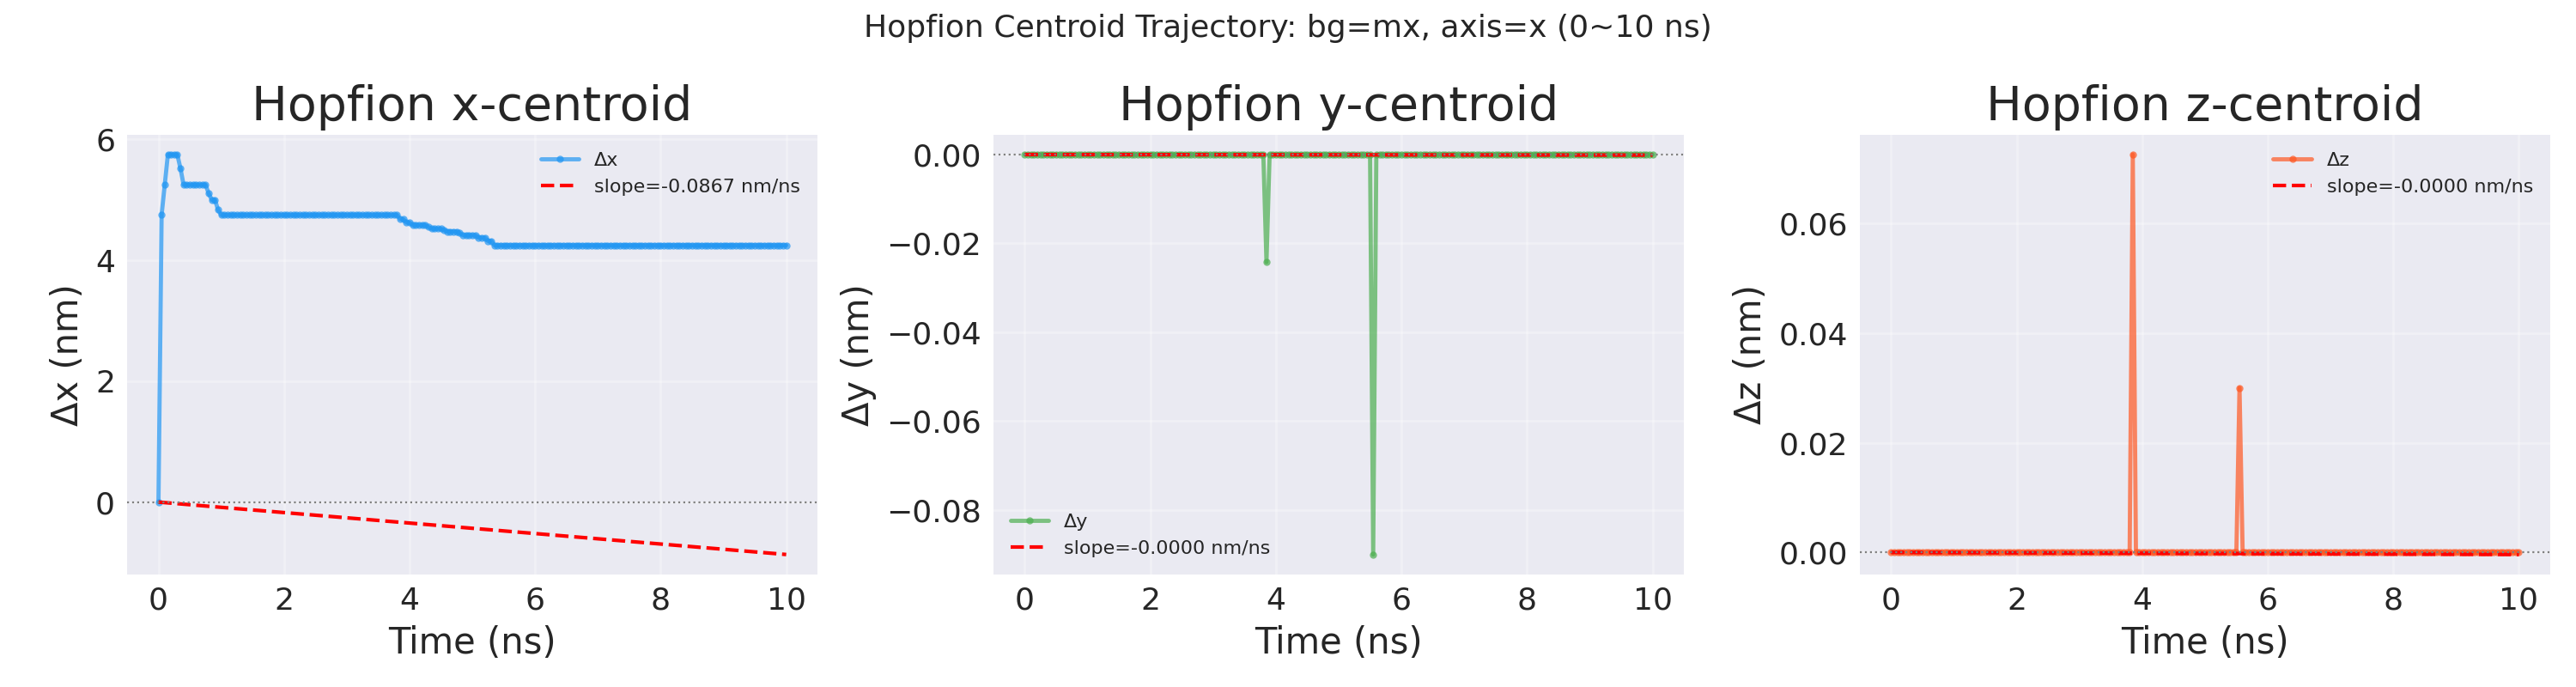
\includegraphics[width=0.95\textwidth]{figures/fig3-4_drift_trajectory_10ns.png}
  \caption{$m_x = +1$ 背景下 Hopfion 的 \SI{10}{ns} 质心轨迹。$x$ 方向（Hopfion 轴向）在前 \SI{1}{ns} 内发生 $\approx\SI{4.75}{nm}$ 一次性格点弛豫后完全钉扎；$y$、$z$ 方向全程零漂移}
  \label{fig:drift-10ns}
\end{figure}

\par\noindent\textbf{居中稳态验证}\par\nobreak

前述漂移分析中，所有 $m_z = +1$ 背景下的 Hopfion 质心都沿 $z$ 方向发生了一次性位移（参见 \cref{tab:drift-results}），弛豫后已经偏离了原本设定的几何中心。这种偏移会直接拖累后续的自旋波仿真：质心靠向吸收边界层，自旋波往往在尚未抵达 Hopfion 核心时就被衰减殆尽。

为绕开这一问题，本研究采用\textbf{周期性平移}策略。借助三维 PBC 的平移不变性，把弛豫后的磁化构型沿 $z$ 轴整体移位，令质心回到盒子几何中心 $(\SI{25}{nm}, \SI{25}{nm}, \SI{25}{nm})$。操作由 NumPy 的 \texttt{np.roll} 完成，磁化分布形态丝毫未变，仅平移其在周期盒中的坐标。

平移后的构型稳定性需要重新校核。本文挑选三组代表性配置（$K_{u1} = 0$、$\SI{10e3}{}$、$\SI{50e3}{J/m^3}$），在 $\alpha = 0.2$、PBC 条件下分别演化 \SI{1}{ns}，持续追踪 Hopfion 质心位置及核心细胞数（$m_z < 0$ 的格点数）。判定口径定在 $z$ 方向漂移 $|\Delta z| < \SI{2}{nm}$。

\cref{tab:centered-stability}给出验证结果。三组配置悉数通过稳态判据，最大漂移仅 $\SI{0.70}{nm}$（$K_{u1} = 0$）；$K_{u1} = \SI{10e3}{J/m^3}$ 时漂移低至 $\SI{0.019}{nm}$，位置稳定性表现极为出色。

\begin{table}[htbp]
  \centering
  \caption{居中 Hopfion 的 \SI{1}{ns} 稳态验证结果}
  \label{tab:centered-stability}
  \begin{tabular}{ccccc}
    \toprule
    $K_{u1}$ (J/m$^3$) & $z_0$ (nm) & $z_{\text{final}}$ (nm) & $\Delta z$ (nm) & 核心细胞数 \\
    \midrule
    0     & 28.44 & 29.15 & $+0.70$ & 1984 $\to$ 2128 \\
    10000 & 25.07 & 25.05 & $-0.019$ & 920 $\to$ 908 \\
    50000 & 25.13 & 25.19 & $+0.062$ & 388 $\to$ 404 \\
    \bottomrule
  \end{tabular}
\end{table}

三组配置的 $z$ 向漂移时间演化参见\cref{fig:centered-z-drift}。$K_{u1} = 0$ 会出现约 $\SI{1}{nm}$ 振幅的呼吸模式振荡，但长时均值仍在可控区间；$K_{u1} = \SI{10e3}{}$ 及 $\SI{50e3}{J/m^3}$ 两组则近乎完全静止。\cref{fig:centered-core-count}呈现核心细胞数的时间演化：较高 $K_{u1}$ 的两组尺寸高度稳定，$K_{u1} = 0$ 的振荡则与其 $z$ 向呼吸模式节拍同步。

综合上述各项指标，$K_{u1} = \SI{10e3}{J/m^3}$ 的居中 Hopfion 在位置稳定性与结构保持两项上均拔得头筹，原先困扰本研究的漂移不确定性由此得以消除。此后本文以居中稳态为起点，考察各向异性参数对 Hopfion 的影响。

\begin{figure}[htbp]
  \centering
  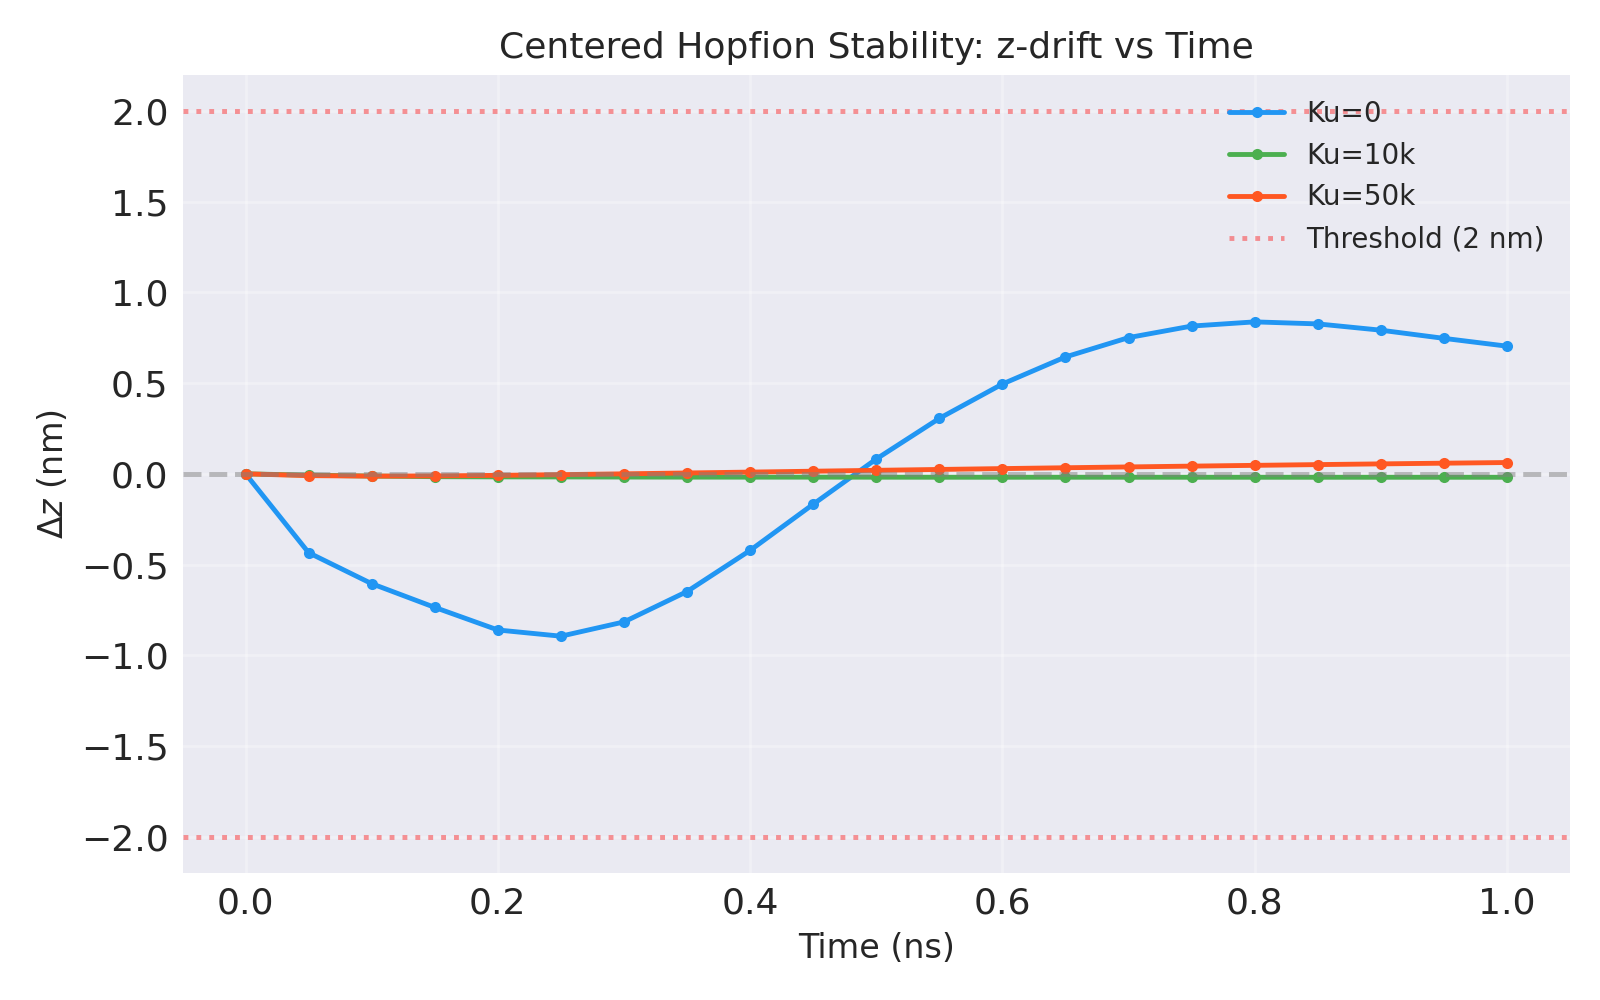
\includegraphics[width=0.85\textwidth]{figures/fig3-8_centered_z_drift.png}
  \caption{居中 Hopfion 的 $z$ 方向漂移随时间演化。虚线标记 $\pm\SI{2}{nm}$ 判定阈值。$K_{u1} = 0$ 表现为呼吸模式振荡，$K_{u1} = \SI{10e3}{}$ 和 $\SI{50e3}{J/m^3}$ 几乎无漂移}
  \label{fig:centered-z-drift}
\end{figure}

\begin{figure}[htbp]
  \centering
  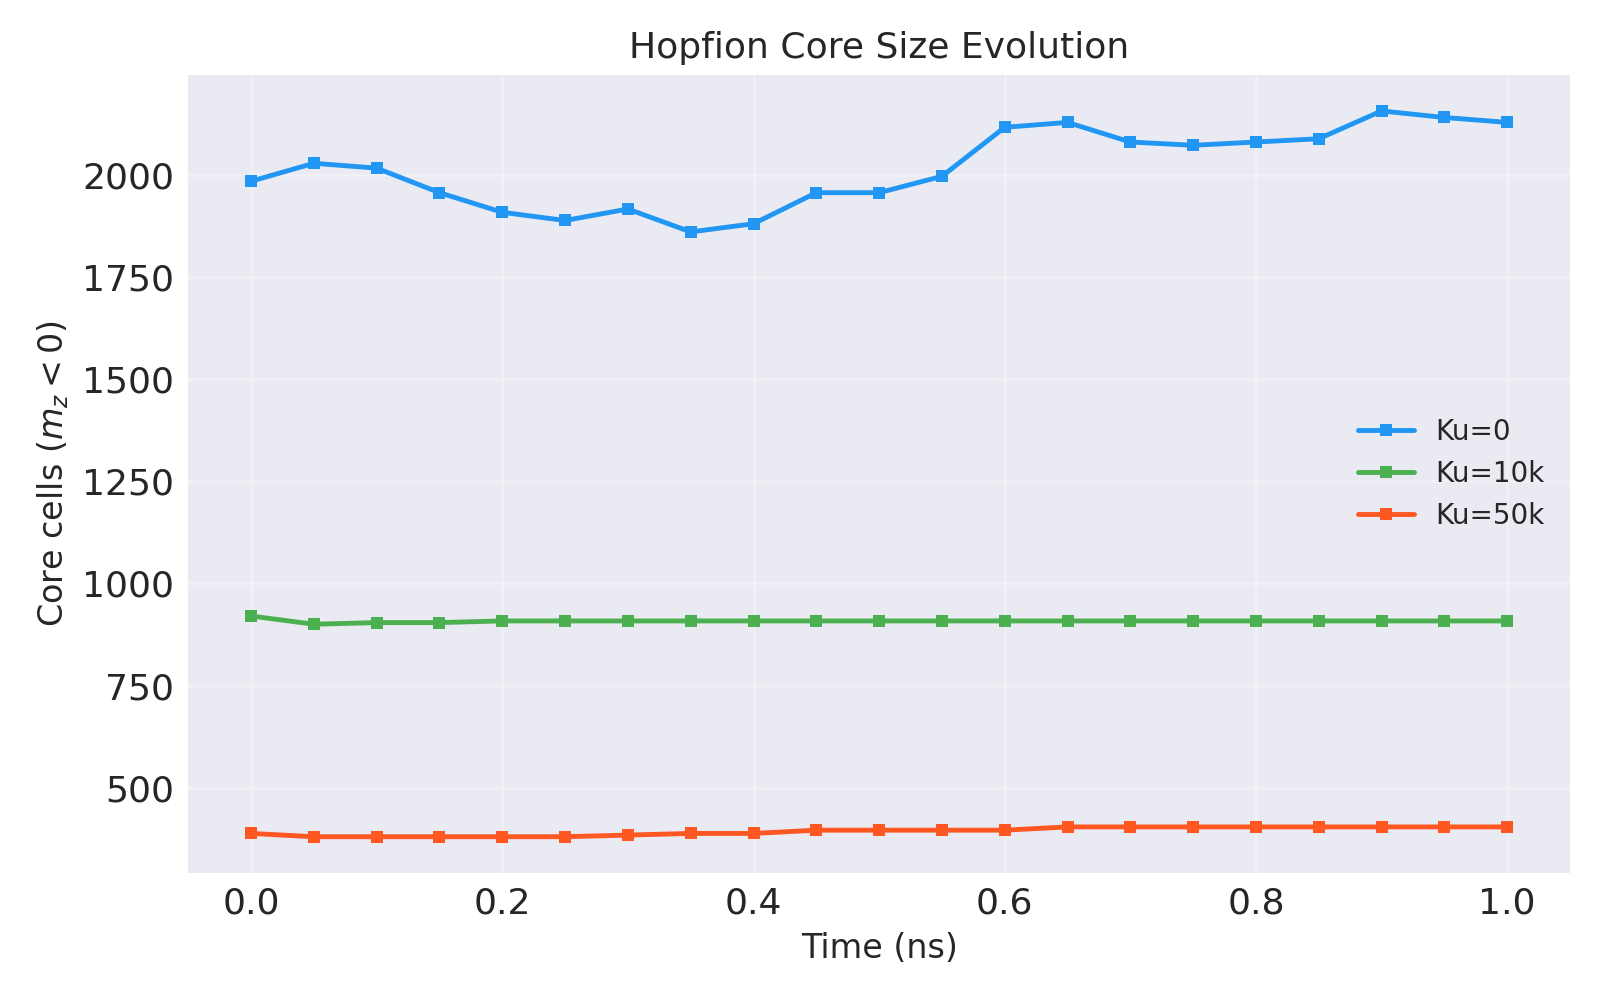
\includegraphics[width=0.85\textwidth]{figures/fig3-9_centered_core_count.png}
  \caption{Hopfion 核心细胞数（$m_z < 0$）随时间演化。各向异性越强，核心越小但越稳定}
  \label{fig:centered-core-count}
\end{figure}


\par\noindent\textbf{各向异性对稳定性的影响}\par\nobreak

本文在竞争交换体系中引入沿 Hopfion 轴向的单轴磁晶各向异性 $K_{u1}$，考察其对已具备居中稳定性的 Hopfion 结构所起的作用。扫描跨度选在 $K_{u1} = 0 \sim \SI{75e3}{J/m^3}$，其中 $\SIrange{50e3}{58e3}{J/m^3}$ 区段加密至 $\SI{1e3}{J/m^3}$ 步长。每组实验以弛豫后的 $R = \SI{8}{nm}$、$r = \SI{4}{nm}$ 构型作为起点，$\alpha = 0.2$ 下各跑 \SI{1}{ns}。

\cref{fig:anisotropy-time}给出各 $K_{u1}$ 取值下 Hopfion 环面半径 $R$ 与管径 $r$ 的时间曲线。从同一初始尺寸出发的所有构型在约 \SI{0.6}{ns} 内收敛到各自的平衡态。随 $K_{u1}$ 上升，平衡的 $R$ 与 $r$ 同步缩小，这反映了各向异性对 Hopfion 结构形成的压缩趋势。

$t = \SI{1}{ns}$ 时刻各组尺寸参数整理于\cref{tab:ku-sweep-large}。$K_{u1} = \SI{52e3}{J/m^3}$ 时 Hopfion 尚能存活，核心体素数从初始的 20344 缩至 376，对应管径约 $\SI{1.2}{nm}$（约 2.4 个格点）。$K_{u1} = \SI{55e3}{J/m^3}$ 时核心体素数归零，Hopfion 彻底坍缩为均匀态。$K_{u1} = \SI{75e3}{J/m^3}$ 更为剧烈，仿真进行到 \SI{0.37}{ns} 便因数值失稳而中断。

\begin{table}[htbp]
  \centering
  \caption{不同 $K_{u1}$ 下 Hopfion 弛豫 \SI{1}{ns} 后的尺寸参数}
  \label{tab:ku-sweep-large}
  \begin{tabular}{cccc}
    \toprule
    $K_{u1}$ (J/m$^3$) & $R$ (nm) & $r$ (nm) & 状态 \\
    \midrule
    0     & 2.63 & 2.22 & 稳定 \\
    5000  & 2.35 & 1.85 & 稳定 \\
    10000 & 2.17 & 1.64 & 稳定 \\
    20000 & 1.82 & 1.54 & 稳定 \\
    30000 & 1.82 & 1.38 & 稳定 \\
    50000 & 1.56 & 1.24 & 稳定 \\
    52000 & 1.50 & 1.20 & 稳定（临界） \\
    55000 & —    & —    & 坍缩 \\
    75000 & —    & —    & 坍缩 \\
    \bottomrule
  \end{tabular}
\end{table}

据此本文划定\textbf{临界各向异性阈值}：
\begin{equation}
  K_{u1,c} \in (\num{52e3}, \, \num{55e3}) \, \si{J/m^3}
  \label{eq:ku-critical}
\end{equation}

这一临界行为，可从能量竞争的角度给出解释。Hopfion 的管径 $r$ 来自三条能量通道的平衡：交换能 $\sim A_{\text{ex}}/r^2$，作用是将管径撑开；竞争交换（$J_2$、$J_4$）施加的拓扑约束，把 $r$ 锚定在固有吸引子尺度附近；各向异性能 $\sim K_{u1} r^2 L$（$L$ 为管长），则沿相反方向挤压反向磁化体积，使管径收缩。

$K_{u1}$ 较小时，拓扑约束与交换能之间的角力主导全局，$r$ 在吸引子附近稳稳停住。随 $K_{u1}$ 攀升，各向异性的收缩作用持续增强。一旦跨过 $K_{u1,c}$，收缩力压过了拓扑抗力，管径被挤到格点分辨率（$\sim \SI{0.5}{nm}$）的量级，离散网格再也撑不起拓扑结构，Hopfion 就此坍缩。此结果与 Metlov 对螺旋磁体中 Hopfion 椭圆稳定性的理论分析在定性层面相吻合\cite{metlov2025elliptical}。\cref{fig:anisotropy-summary}呈现 $R$、$r$ 随 $K_{u1}$ 单调下降的走势和临界区间的位置。

\begin{figure}[htbp]
  \centering
  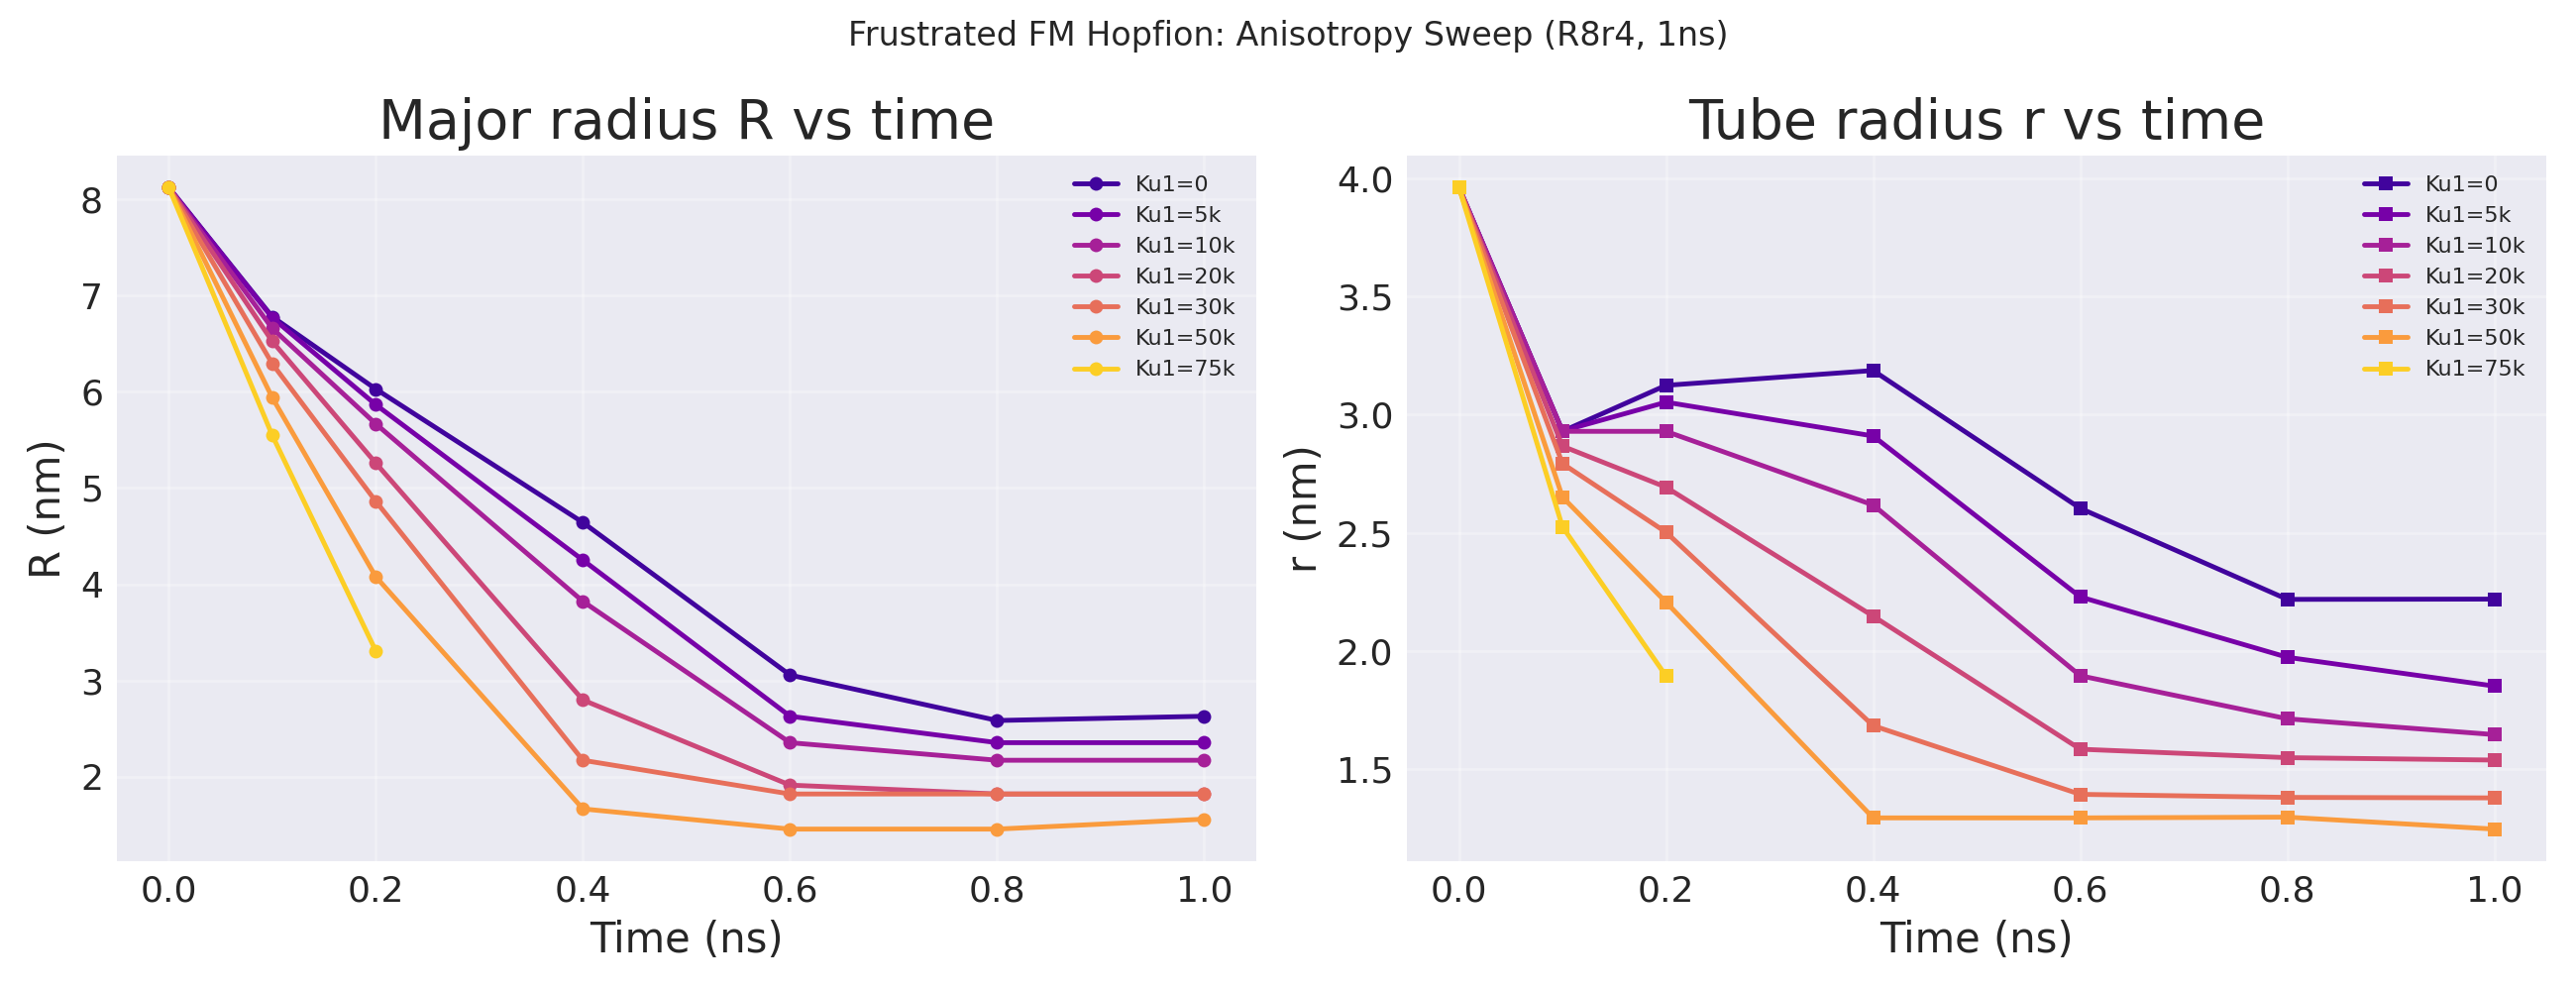
\includegraphics[width=0.95\textwidth]{figures/fig3-6_anisotropy_Rr_vs_time.png}
  \caption{不同 $K_{u1}$ 下 Hopfion 尺寸参数 $R(t)$ 和 $r(t)$ 的时间演化。所有构型从 $R = \SI{8}{nm}$, $r = \SI{4}{nm}$ 出发，$K_{u1}$ 增大导致平衡尺寸持续缩小。$K_{u1} = \SI{75e3}{J/m^3}$ 仅有前 3 帧数据，仿真因 Hopfion 坍缩而中断}
  \label{fig:anisotropy-time}
\end{figure}

\begin{figure}[htbp]
  \centering
  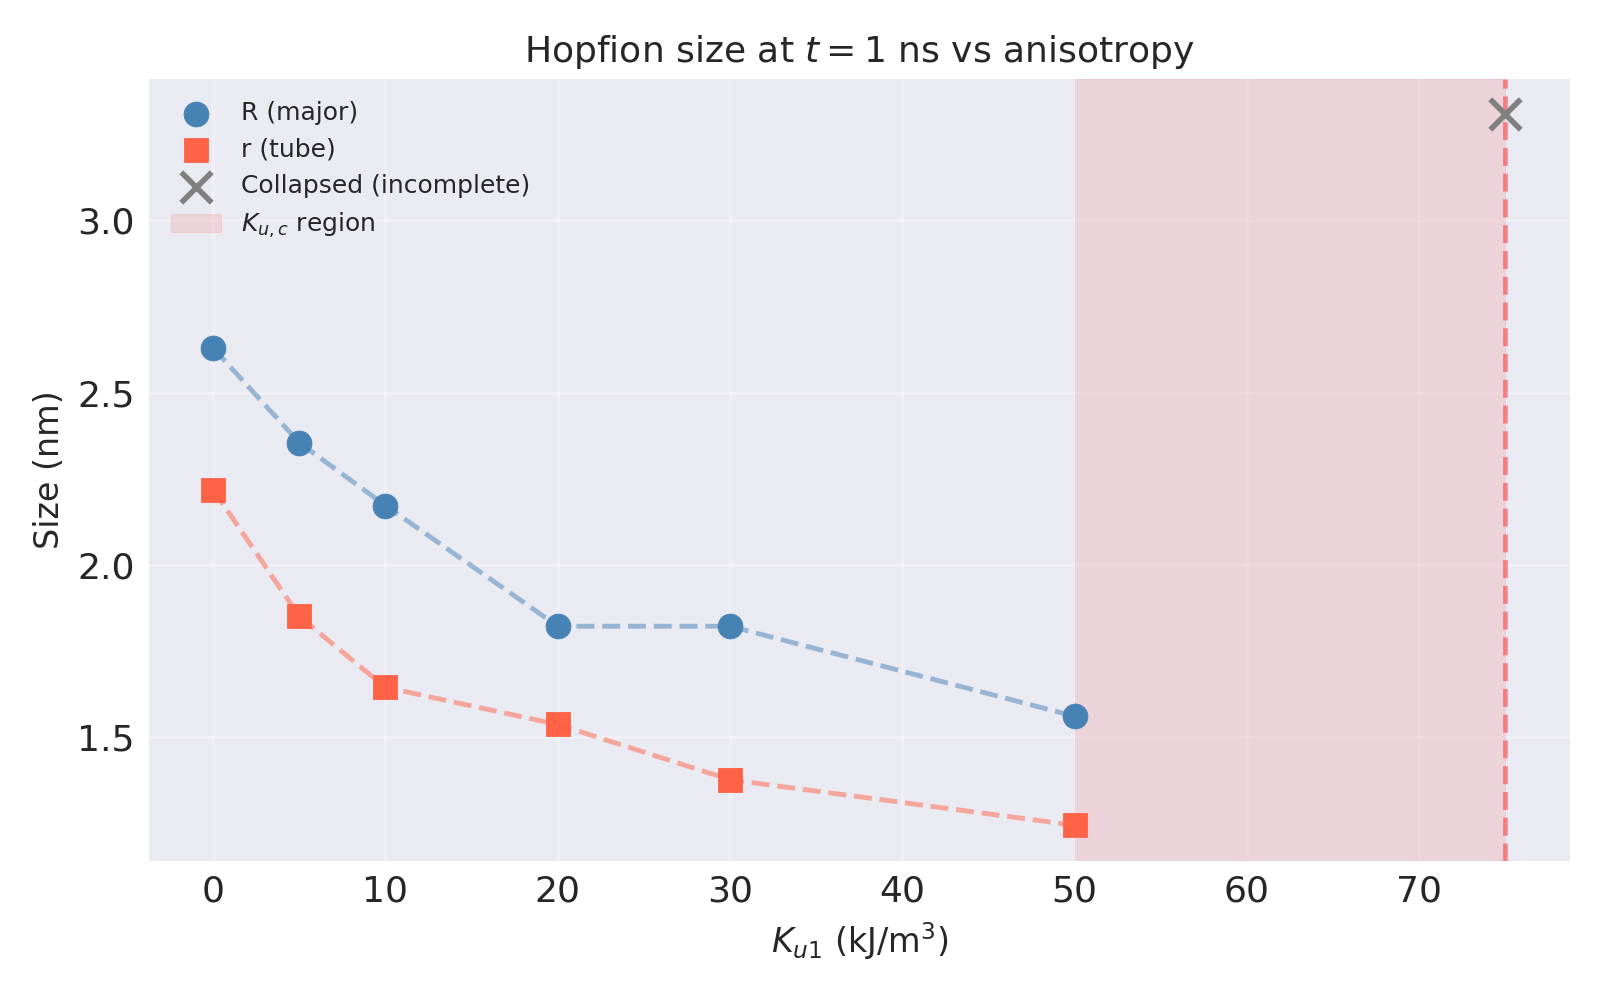
\includegraphics[width=0.8\textwidth]{figures/fig3-7_anisotropy_summary.png}
  \caption{$t = \SI{1}{ns}$ 时 Hopfion 尺寸参数随 $K_{u1}$ 的变化。红色阴影区域标记临界阈值 $K_{u1,c} \in (\num{52e3}, \num{55e3}) \, \si{J/m^3}$，灰色叉号表示 Hopfion 已坍缩}
  \label{fig:anisotropy-summary}
\end{figure}

\par\noindent\textbf{固有尺寸吸引子}\par\nobreak

为判断 Hopfion 弛豫后的平衡尺寸是否受初始条件牵制，本文展开了尺寸收敛性测试。具体做法是以不同初始尺寸（环面半径 $R$ 和管径 $r$）构造若干 Hopfion 初始态，在 $\alpha = 5.0$ 的高阻尼下弛豫至稳态，然后用 Python 脚本提取弛豫后的几何参数。

\cref{fig:size-convergence}呈现收敛测试的结果。不管初始尺寸怎样设置（$R = 3 \sim \SI{12}{nm}$, $r = 2 \sim \SI{5}{nm}$），弛豫后的 Hopfion 都汇聚到同一平衡尺寸：
\begin{equation}
  R_{\text{eq}} = \SI{2.60}{nm}, \quad r_{\text{eq}} = \SI{2.16}{nm}
  \label{eq:attractor}
\end{equation}

这说明在本文所用参数下，系统确实拥有一个唯一的\textbf{固有尺寸吸引子}：Hopfion 的平衡几何由材料参数单独决定，与初始选取无关。这也解释了为何在某一固定的各向异性参数配套下，对应的稳态只会对应一种固定特征的 Hopfion 尺寸。整体权衡下来，$K_{u1} = \SI{10e3}{J/m^3}$ 且处于居中位置的 Hopfion 在多个指标上均最为出色，本文即将其选作后续自旋波驱动仿真（第五章）的初始态。

\begin{figure}[htbp]
  \centering
  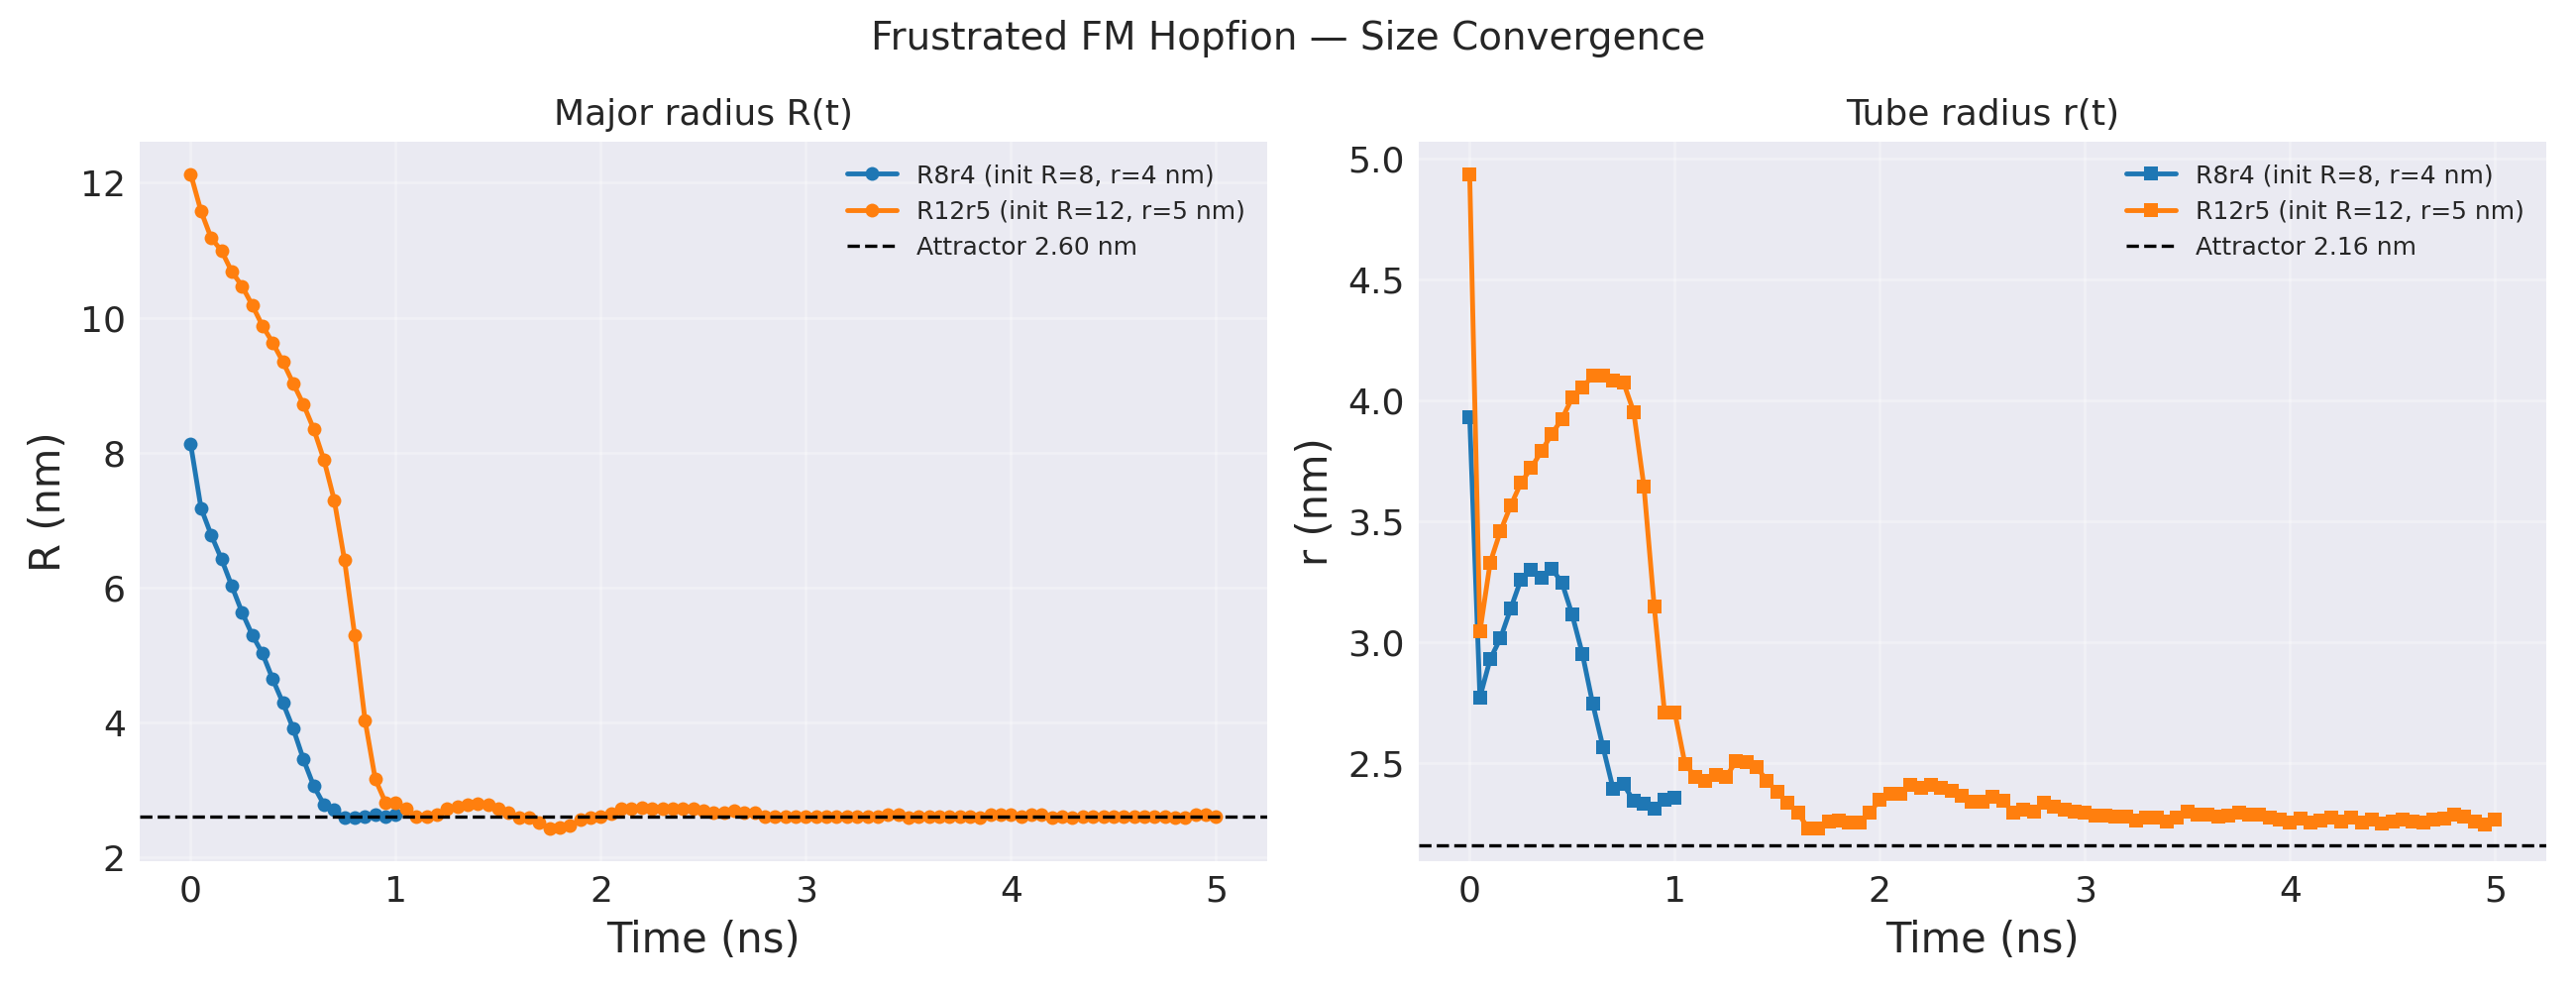
\includegraphics[width=0.95\textwidth]{figures/fig3-3_size_convergence.png}
  \caption{尺寸收敛性测试。不同初始尺寸（$R = 8, \SI{12}{nm}$）的 Hopfion 弛豫后均收敛至相同的平衡尺寸 $R_{\text{eq}} = \SI{2.60}{nm}$, $r_{\text{eq}} = \SI{2.16}{nm}$，证实固有尺寸吸引子的存在}
  \label{fig:size-convergence}
\end{figure}


针对 Hopfion 的稳定边界问题，本章覆盖两类铁磁介质并给出四条可验证结论：

\begin{enumerate}[label=(\arabic*)]
  \item 对于 DMI 铁磁（FeGe）一路，Hopfion 的存活需要解析初始态、边界层冻结与退磁场效应三项条件同时满足；在此组合下，$d = 3\lambda$、$h = \lambda$ 的圆柱模型可稳定演化 \SI{2}{ns}。
  \item 竞争交换铁磁体系下，控制变量组实验排除了一项此前的猜想——背景磁化取向与 Hopfion 漂移行为解耦，四组配置展现出一致的轴向初始漂移。
  \item 在此判据基础上，本文先用周期性平移把 Hopfion 居中、再以 \SI{1}{ns} 二次验证，确认了 $m_z$ 背景下的位置稳定性；随后的细化扫描把临界各向异性阈值限定在 $K_{u1,c} \in (\num{52e3}, \num{55e3}) \, \si{J/m^3}$ 区间。
  \item 最后一项结论涉及固有尺寸吸引子——Hopfion 的平衡几何由各向异性等材料参数唯一确定；从多组对比来看，$K_{u1} = \SI{10e3}{J/m^3}$ 的居中构型表现最优（$\Delta z = \SI{0.019}{nm}$），本文据此选定它作为第五章自旋波仿真的初始态。
\end{enumerate}

上述判据与参数组合为第五章的动力学调控研究提供了直接可用的起点——$K_{u1} = \SI{10e3}{J/m^3}$ 与居中构型将沿用至自旋波驱动实验。
